\section{On-accelerator training framework} \label{sec:framework}
In contrast to the typical offline training framework on GPPs, we propose an 
on-accelerator training framework to allow the CNN accelerator's runtime variation 
caused by approximate arithmetic logic, overclocking or soft errors 
to be learned with the application data. With the on-accelerator training,
the obtained model can be deployed despite the accelerator's 
undeterministic behavior. Details of the framework will be presented in 
the rest of this section.

\begin{figure*}
        \center{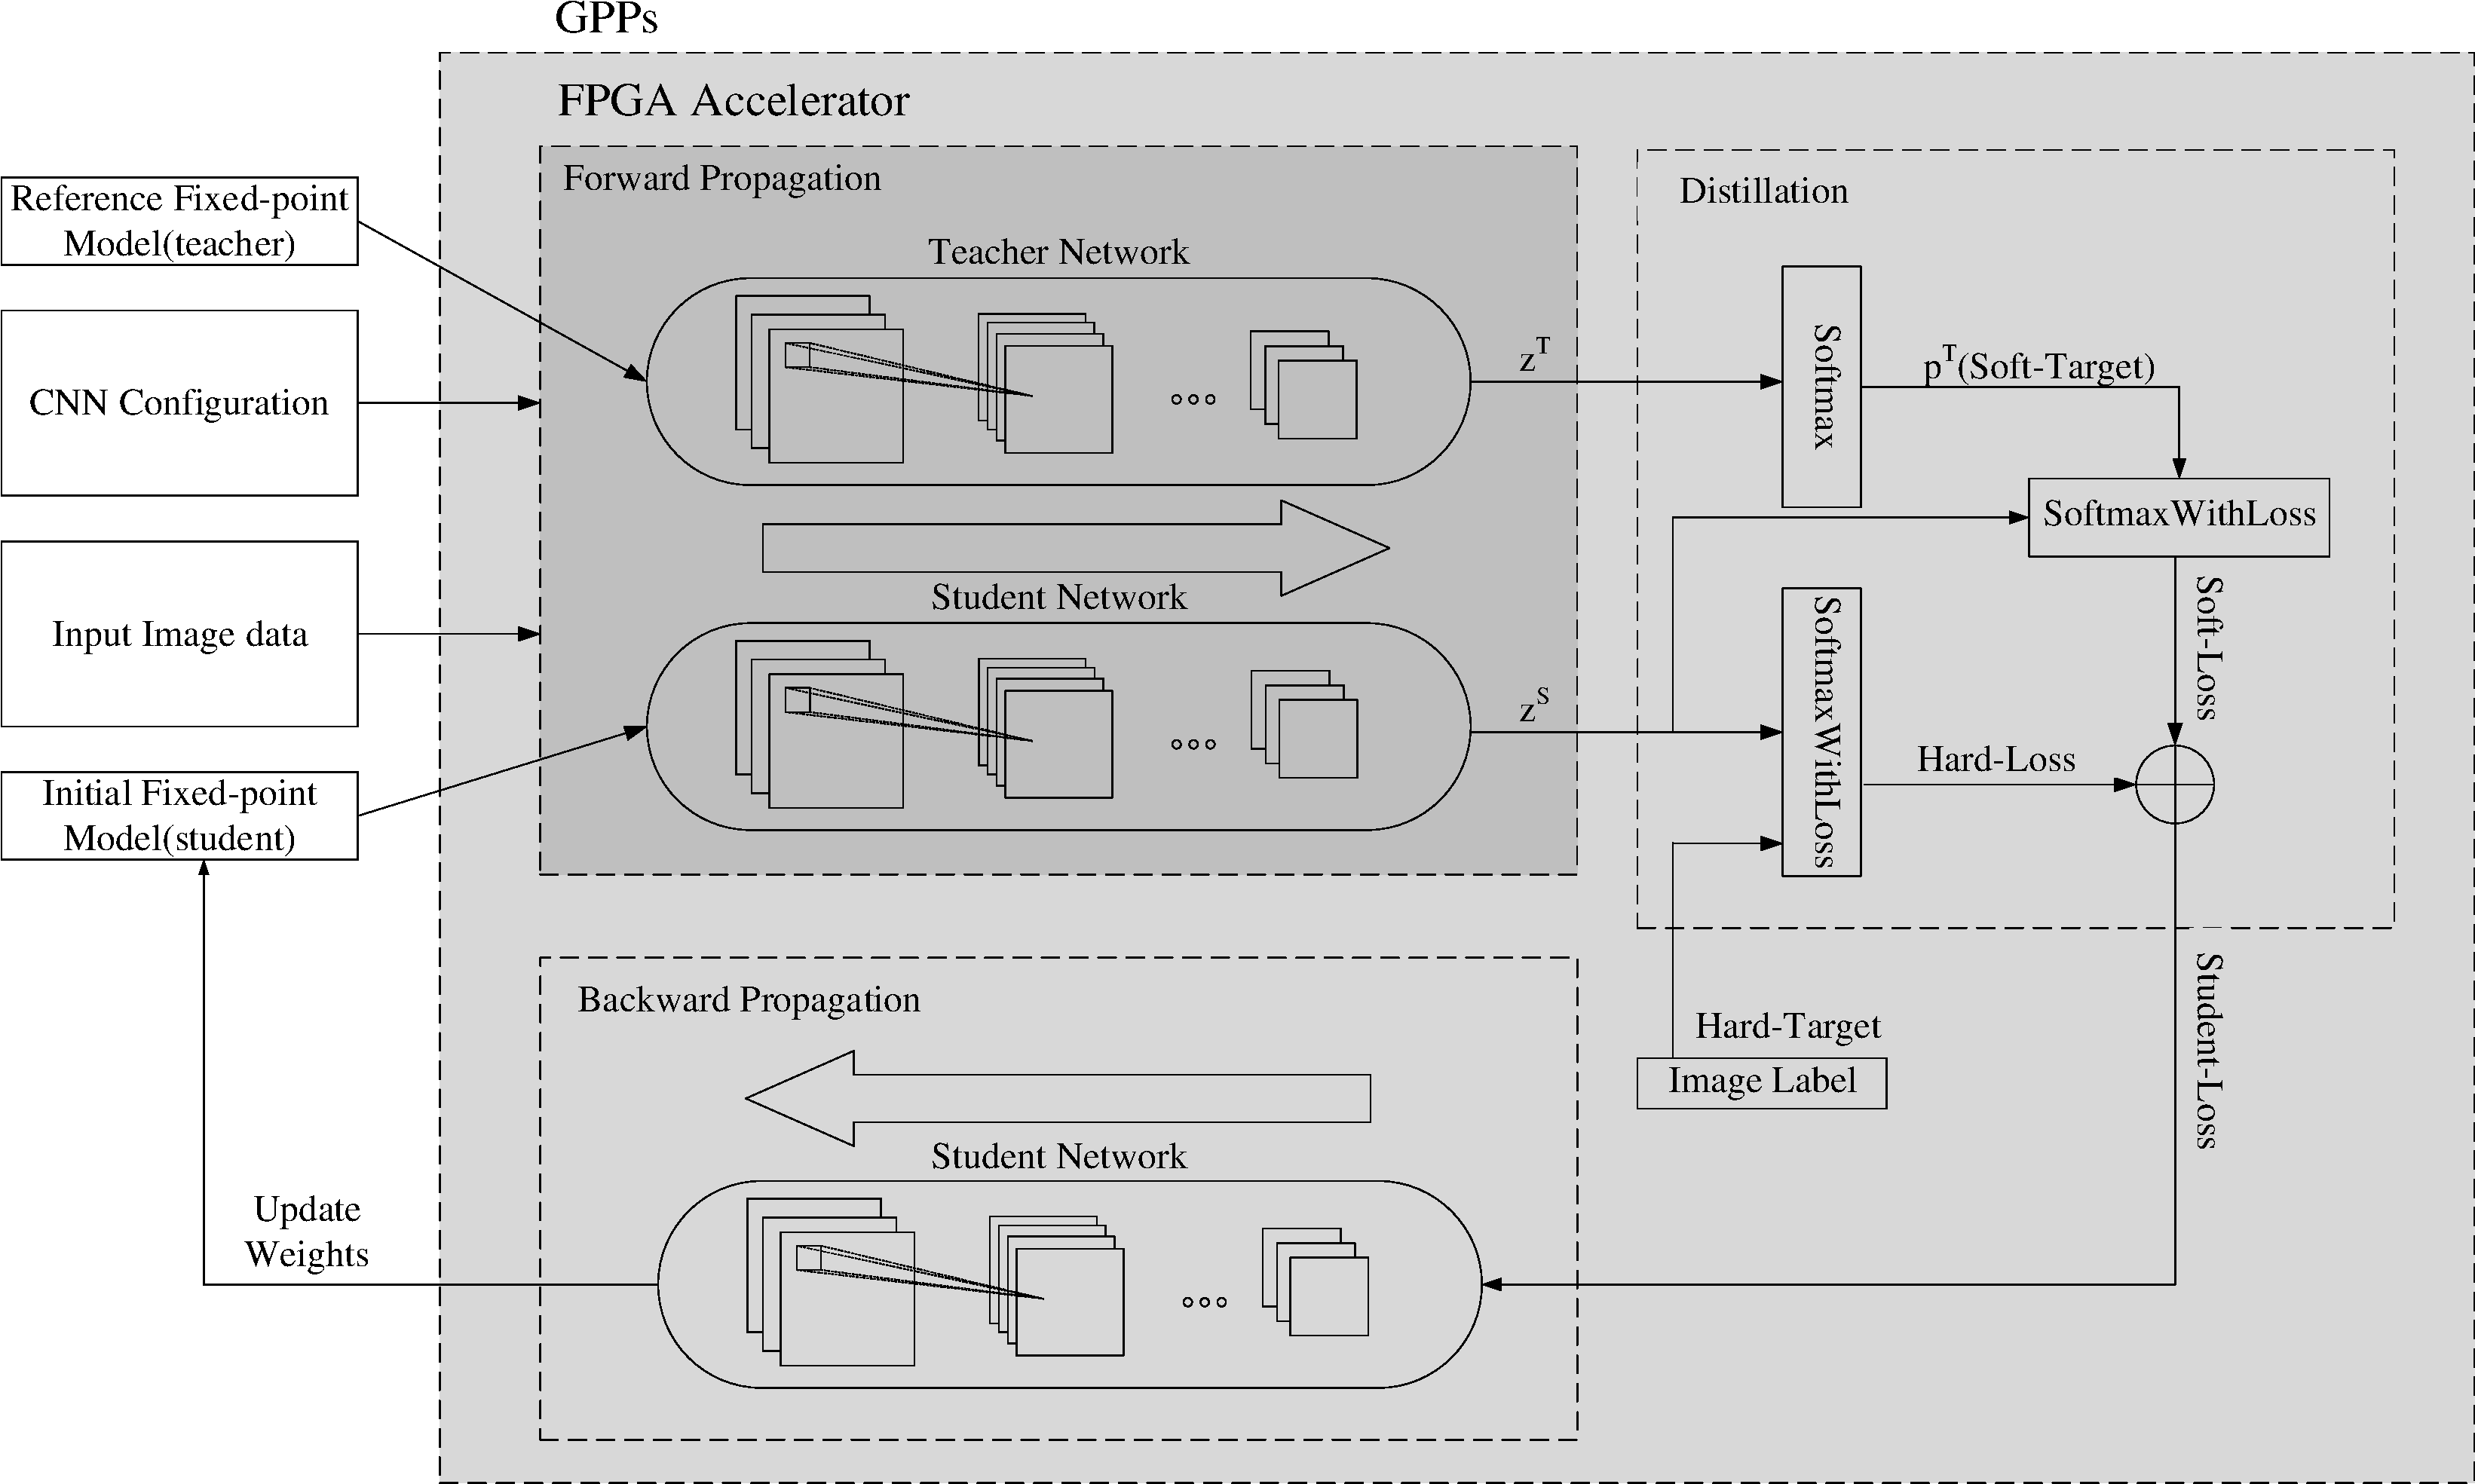
\includegraphics[width=0.85\linewidth]{retrain}}
        \caption{On-accelerator training framework with knowledge distilling}
        \label{fig:retrain}
%        \vspace{-0.5em}
\end{figure*}


\subsection{Overall training framework}
The on-accelerator training is essentially to have the neural 
network models to tolerate the accelerators' dynamic variation. 
While the variation is similar to the quantization 
errors in certain extent, the ideal network model can be 
close to the pretrained neural network model in terms of 
network structure. In this case, we borrow the idea of knowledge 
distilling\cite{distillation_38, distillation_39}, 
which can be used to have a high-precision neural network to teach a 
low-precision neural network with similar network structure efficiently, 
for the on-accelerator training. Basically, the offline pretrained 
model can be regarded as a teacher model and used to guide the training of the 
student model with lower precision. After the training, the student model 
can perform much better despite the accelerators' computing variation.


With the knowledge distilling strategy, we develop an on-accelerator training 
framework as illustrated in Figure \ref{fig:retrain}. The framework roughly consists of three parts
including forward propagation, knowledge distilling and backward propagation. 
Both the teacher network and the student network will go through the 
forward propagation. The computing results i.e. $z^T$ and $z^S$ in 
combination with the label of the input image data will be fed to the 
knowledge distilling part. In the knowledge distilling part,  
the logit of softmax i.e. $z^T$ and $z^S$ are further used to calculate the 
softmax i.e. $p^T$ and $p^S$ with Equation \ref{eq:pt-calu}. 
Note that the logit of the teacher network is divided by a 
temperature factor t. It can be used to adjust the softmax 
probability distribution. Using a higher value for t 
produces a softer probability distribution and stresses 
the training process. 

On top of the softmax, we can further calculate the student 
network loss with Equation \ref{eq:student-loss}. It includes 
two different parts i.e.$L(y, p^S)$ and $L(p^T, p^S)$ which can be 
obtained with Equation \ref{eq:loss}. The student loss is used in the 
back propagation part as conventional neural network training. 
After the back propagation, weights will be updated and used for the 
next training iteration. The training will stop when the prediction 
accuracy gets converged.

\begin{equation}
	\label{eq:pt-calu}
p_j=\frac{e^{{z_j}/t}}{\sum_{i=1}^{K}e^{{z_i}/t}}
\end{equation}

\begin{equation}
	\label{eq:student-loss}
L=\alpha*L(y,p^S)+\beta*L(p^T,p^S)
\end{equation}

\begin{equation}
	\label{eq:loss}
L(y,p)=-\sum_{i=1}^{K}y_i*log(p_i)
\end{equation}


To make the training aware the accelerators' dynamic variation, 
we have the forward propagation of the student network 
performed on the accelerator directly while the rest of the 
framework remains on GPPs. The forward propagation on 
the accelerator is fixed point. The backward propagation on 
GPPs adopts the floating point to ensure 
the small change in the gradient can be accumulated \cite{Matthieu2014_8}. 
Otherwise, the gradient may disappear due to the 
quantization and new infomration can no longer be learned.

\begin{table*}
        \centering
        \vspace{-0.3em}
        \caption{High-level interface to integrate general CNN accelerators with Caffe}
        \label{tab:api}
        \vspace{-0.3em}
        \begin{tabular}{c|l|l}
                \toprule
                ID & Function Name & Description  \\
                \midrule
                1 & launchAccelerator() & It configures the CNN accelerator and launches it from host CPU. \\
		\midrule
                2 & dataToFPGA(weight, input, wgtDevAddr, inDevAddr) & It transfers both the input data and weight to the FPGA device memory. \\
		\midrule
		3 & dataFromFPGA(outputDevAddr, output) & \shortstack[l]{It transfers all the intermediate output of the CNN layers from FPGA \\device memory to host memory.} \\
		\midrule
		4 & convertIntToFloat(int iData, float fData) & It converts the fixed-point output to float for back propagation processing. \\
		\midrule
		5 & convertFloatToInt(float fData,  int iData) & \shortstack[l]{It converts the floating-point input and weight data to fixed point or \\integer for forward processing on the accelerator.} \\
		\midrule
		6 & dataLayoutReorder(data, reorderedData) & \shortstack[l]{It reorders the data layout for more efficient accelerator execution before \\sending to FPGA device memory.} \\
		\midrule
		7 & dataLayoutRecover(reorderedData, data) & It reorders the output data back to the default format for Caffe back propagation. \\
                \bottomrule
        \end{tabular}
        \vspace{-1em}
\end{table*}



\subsection{CNN accelerator abstraction}
As illustrated in the above section, the forward propagation of the 
student network will be executed on the CNN accelerator while 
the rest part runs on GPPs. Essentially, the framework targets at a 
heterogeneous computing architecture and frequent 
communication between the accelerator and the GPPs is expected. 
In order to fit various CNN accelerators within the same training framework,
we abstract the CNN accelerators with a high-level interface
which makes the accelerators near transparent to the training framework.

Centering the data communication between the forward propagation 
and the rest of the training framework, we define a high-level 
interface which consists of 7 functions as listed in Table \ref{tab:api}. 
Function 1 is used to launch the CNN accelerator from host. 
Function 2 and 3 are used to transfer data between the host memory and the device memory during 
the training. As the forward propagation on the CNN accelerators is usually fixed point 
and the back propagation on GPPs is floating point, data type converting between fixed point 
and floating point is required. Function 4 and 5 can be used for this purpose. 
Function 1 to 5 are required for all the accelerators. 
Function 6 and 7 are only used for accelerators that compute on reorganized data\cite{pipecnn_2,deepburing_12}. 
With the interface functions, general CNN accelerators can be conveniently 
referenced and used in the proposed on-accelerator training framework. 

In this work, we have the CNN accelerator implemented on Xilinx FPGAs as a case study. 
With Xilinx SDAccel, we can wrap the accelerators with OpenCL API while the accelerators 
can either be developed with OpenCL, HLS or RTL. On top of the OpenCL API, the proposed 
high-level interface can be implemented. Meanwhile, we use Caffe, a C++ based 
deep learning framework, to construct the on-accelerator training framework. With 
both parts developed with C family languages, they can be integrated conveniently. 

%In this work, we have the CNN accelerator implemented on FPGAs.
%Figure 4 depicts the implementation of the training framework on a hybrid 
%CPU-FPGA architecture. In this work, we use Xilinx KCU1500 as the FPGA board 
%and put it on a standard desktop computer. CPU is the controller and it reconfigures 
%the accelerator for a specific CNN structure. In each training iteration, CPU launches 
%the CNN accelerator to perform the forward propagation from bottom layer to top layer. 
%CPU does the backward propagation from top layer to bottom layer. Weights and the image 
%data are initially stored in host memory. It will be transferred to FPGA offchip memory 
%for forward propagation through PCI-E. Similarly, the output data will be transferred 
%from FPGA off-chip memory back to host memory after forward propagation. Because of the 
%OpenCL based API wrapper in SDAccel, the CNN accelerator’s interface can be easily 
%exposed to Caffe for referring to the forward propagation result. 


\subsection{CNN accelerator modification}
On top of the high-level interface, the CNN accelerator also needs 
minor adjustments to enable the on-accelerator training. 
Typically, the training requires the feature map of each neural 
network layer for backward propagation. However, many of the accelerators 
are intensively optimized for inference only and some of the layers’ output 
are fully buffered in on-chip memory to reduce the external memory access. 
In this case, the accelerator should provide an optional data path such that 
intermediate output data can be written to external memory at request.
As shown in Figure \ref{fig:change_of_accelerator}, the output of each layer 
will be transferred to memory using the added optional data path 
when the accelerator is used for training. The write back data path 
can be switched off when the accelerator is used for inference. 
It is trivial to modify the CNN accelerators and the hardware
resource consumption is negligible.

\begin{figure}
        \center{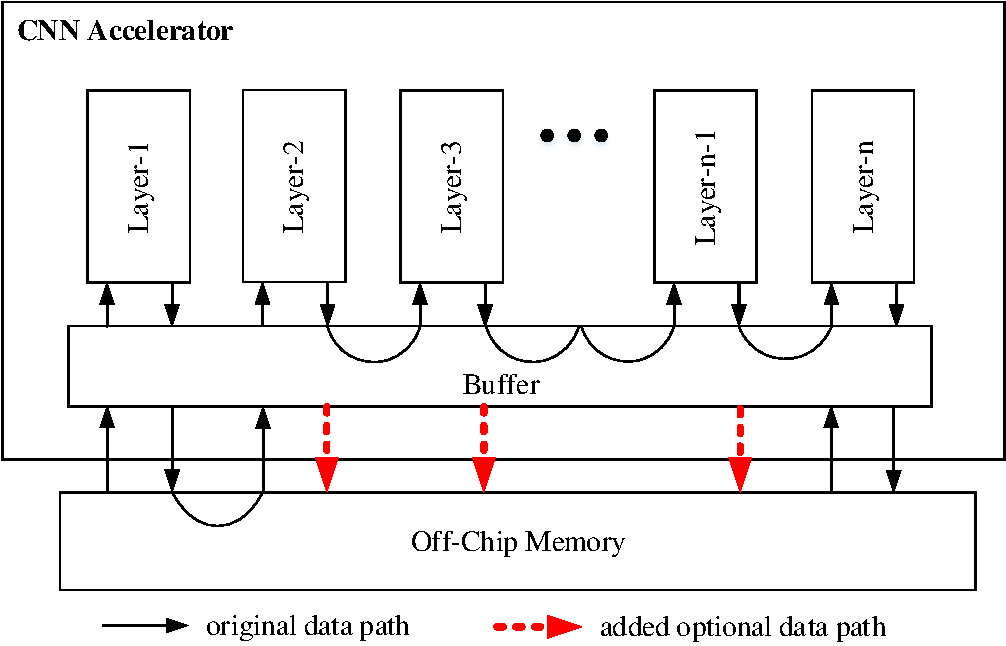
\includegraphics[width=0.85\linewidth]{change_of_accelerator}}
        \caption{Modification of the CNN accelerator data path. It essentially
ensures the feature map of each neural network layer to have an optional data path 
to external memory for back propagation in training.}
        \label{fig:change_of_accelerator}
        \vspace{-1em}
\end{figure}


